% Options for packages loaded elsewhere
\PassOptionsToPackage{unicode}{hyperref}
\PassOptionsToPackage{hyphens}{url}
%
\documentclass[
  english,
  man]{apa7}
\usepackage{lmodern}
\usepackage{amsmath}
\usepackage{ifxetex,ifluatex}
\ifnum 0\ifxetex 1\fi\ifluatex 1\fi=0 % if pdftex
  \usepackage[T1]{fontenc}
  \usepackage[utf8]{inputenc}
  \usepackage{textcomp} % provide euro and other symbols
  \usepackage{amssymb}
\else % if luatex or xetex
  \usepackage{unicode-math}
  \defaultfontfeatures{Scale=MatchLowercase}
  \defaultfontfeatures[\rmfamily]{Ligatures=TeX,Scale=1}
\fi
% Use upquote if available, for straight quotes in verbatim environments
\IfFileExists{upquote.sty}{\usepackage{upquote}}{}
\IfFileExists{microtype.sty}{% use microtype if available
  \usepackage[]{microtype}
  \UseMicrotypeSet[protrusion]{basicmath} % disable protrusion for tt fonts
}{}
\makeatletter
\@ifundefined{KOMAClassName}{% if non-KOMA class
  \IfFileExists{parskip.sty}{%
    \usepackage{parskip}
  }{% else
    \setlength{\parindent}{0pt}
    \setlength{\parskip}{6pt plus 2pt minus 1pt}}
}{% if KOMA class
  \KOMAoptions{parskip=half}}
\makeatother
\usepackage{xcolor}
\IfFileExists{xurl.sty}{\usepackage{xurl}}{} % add URL line breaks if available
\IfFileExists{bookmark.sty}{\usepackage{bookmark}}{\usepackage{hyperref}}
\hypersetup{
  pdftitle={Development of an Intended Bifactor Engagement Measure},
  pdfauthor={Morgan Russell1, Casey Osorio-Duffoo2, Renata Garcia Prieto Palacios Roji1, \& John Kulas1},
  pdflang={en-EN},
  pdfkeywords={Engagement, bifactor analysis},
  hidelinks,
  pdfcreator={LaTeX via pandoc}}
\urlstyle{same} % disable monospaced font for URLs
\usepackage{graphicx}
\makeatletter
\def\maxwidth{\ifdim\Gin@nat@width>\linewidth\linewidth\else\Gin@nat@width\fi}
\def\maxheight{\ifdim\Gin@nat@height>\textheight\textheight\else\Gin@nat@height\fi}
\makeatother
% Scale images if necessary, so that they will not overflow the page
% margins by default, and it is still possible to overwrite the defaults
% using explicit options in \includegraphics[width, height, ...]{}
\setkeys{Gin}{width=\maxwidth,height=\maxheight,keepaspectratio}
% Set default figure placement to htbp
\makeatletter
\def\fps@figure{htbp}
\makeatother
\setlength{\emergencystretch}{3em} % prevent overfull lines
\providecommand{\tightlist}{%
  \setlength{\itemsep}{0pt}\setlength{\parskip}{0pt}}
\setcounter{secnumdepth}{5}
% Make \paragraph and \subparagraph free-standing
\ifx\paragraph\undefined\else
  \let\oldparagraph\paragraph
  \renewcommand{\paragraph}[1]{\oldparagraph{#1}\mbox{}}
\fi
\ifx\subparagraph\undefined\else
  \let\oldsubparagraph\subparagraph
  \renewcommand{\subparagraph}[1]{\oldsubparagraph{#1}\mbox{}}
\fi
% Manuscript styling
\usepackage{upgreek}
\captionsetup{font=singlespacing,justification=justified}

% Table formatting
\usepackage{longtable}
\usepackage{lscape}
% \usepackage[counterclockwise]{rotating}   % Landscape page setup for large tables
\usepackage{multirow}		% Table styling
\usepackage{tabularx}		% Control Column width
\usepackage[flushleft]{threeparttable}	% Allows for three part tables with a specified notes section
\usepackage{threeparttablex}            % Lets threeparttable work with longtable

% Create new environments so endfloat can handle them
% \newenvironment{ltable}
%   {\begin{landscape}\centering\begin{threeparttable}}
%   {\end{threeparttable}\end{landscape}}
\newenvironment{lltable}{\begin{landscape}\centering\begin{ThreePartTable}}{\end{ThreePartTable}\end{landscape}}

% Enables adjusting longtable caption width to table width
% Solution found at http://golatex.de/longtable-mit-caption-so-breit-wie-die-tabelle-t15767.html
\makeatletter
\newcommand\LastLTentrywidth{1em}
\newlength\longtablewidth
\setlength{\longtablewidth}{1in}
\newcommand{\getlongtablewidth}{\begingroup \ifcsname LT@\roman{LT@tables}\endcsname \global\longtablewidth=0pt \renewcommand{\LT@entry}[2]{\global\advance\longtablewidth by ##2\relax\gdef\LastLTentrywidth{##2}}\@nameuse{LT@\roman{LT@tables}} \fi \endgroup}

% \setlength{\parindent}{0.5in}
% \setlength{\parskip}{0pt plus 0pt minus 0pt}

% \usepackage{etoolbox}
\makeatletter
\patchcmd{\HyOrg@maketitle}
  {\section{\normalfont\normalsize\abstractname}}
  {\section*{\normalfont\normalsize\abstractname}}
  {}{\typeout{Failed to patch abstract.}}
\patchcmd{\HyOrg@maketitle}
  {\section{\protect\normalfont{\@title}}}
  {\section*{\protect\normalfont{\@title}}}
  {}{\typeout{Failed to patch title.}}
\makeatother
\shorttitle{BiFactor Engagement}
\keywords{Engagement, bifactor analysis\newline\indent Word count: X}
\DeclareDelayedFloatFlavor{ThreePartTable}{table}
\DeclareDelayedFloatFlavor{lltable}{table}
\DeclareDelayedFloatFlavor*{longtable}{table}
\makeatletter
\renewcommand{\efloat@iwrite}[1]{\immediate\expandafter\protected@write\csname efloat@post#1\endcsname{}}
\makeatother
\usepackage{csquotes}
\ifxetex
  % Load polyglossia as late as possible: uses bidi with RTL langages (e.g. Hebrew, Arabic)
  \usepackage{polyglossia}
  \setmainlanguage[]{english}
\else
  \usepackage[shorthands=off,main=english]{babel}
\fi
\ifluatex
  \usepackage{selnolig}  % disable illegal ligatures
\fi
\newlength{\cslhangindent}
\setlength{\cslhangindent}{1.5em}
\newlength{\csllabelwidth}
\setlength{\csllabelwidth}{3em}
\newenvironment{CSLReferences}[2] % #1 hanging-ident, #2 entry spacing
 {% don't indent paragraphs
  \setlength{\parindent}{0pt}
  % turn on hanging indent if param 1 is 1
  \ifodd #1 \everypar{\setlength{\hangindent}{\cslhangindent}}\ignorespaces\fi
  % set entry spacing
  \ifnum #2 > 0
  \setlength{\parskip}{#2\baselineskip}
  \fi
 }%
 {}
\usepackage{calc}
\newcommand{\CSLBlock}[1]{#1\hfill\break}
\newcommand{\CSLLeftMargin}[1]{\parbox[t]{\csllabelwidth}{#1}}
\newcommand{\CSLRightInline}[1]{\parbox[t]{\linewidth - \csllabelwidth}{#1}\break}
\newcommand{\CSLIndent}[1]{\hspace{\cslhangindent}#1}

\title{Development of an Intended Bifactor Engagement Measure}
\author{Morgan Russell\textsuperscript{1}, Casey Osorio-Duffoo\textsuperscript{2}, Renata Garcia Prieto Palacios Roji\textsuperscript{1}, \& John Kulas\textsuperscript{1}}
\date{}


\authornote{

Title: 85 characters;
Abstract: 600 characters
Word count: 3,000 words
Remove names

Correspondence concerning this article should be addressed to Morgan Russell, 1 Normal Ave, Montclair, NJ 07043. E-mail: \href{mailto:russellm5@montclair.edu}{\nolinkurl{russellm5@montclair.edu}}

}

\affiliation{\vspace{0.5cm}\textsuperscript{1} Montclair State University\\\textsuperscript{2} Harver}

\abstract{
Employee engagement has enjoyed a surge in interest as a sought-after attitude despite continued disageement regarding its internal structure and nomological relationship to other constructs, such as satisfaction and burnout. We describe the development of an intentional bi-factor measure of engagement, and document two independent scale definition procedures, one based on internal consistency and the other informed by CFA modification indices. Ultimately, we arrive at scale definitions that should be considered of interest to Industrial and Organizational Psychologists.
}



\begin{document}
\maketitle

Within the context of work, the term ``engagement'' first emerged in the organizational psychology and business literature in the early 1990s (Kahn, 1990). The evolution of the construct can perhaps be considered through the lens of semi-distinct lines of research focused on: 1) work engagement, 2) personal engagement, and 4) employee engagement, and 4) burnout. These perspectives can be identified by slightly differing definitions (and subsequently measures), and perhaps contribute to some confusion regarding what exactly is being measured when organizations survey their employees to assess ``engagement.'' Although ``personal engagement'' was coined in Kahn (1990) , few subsequent articles reference engagement by this name. Schaufeli (2013) distinguishes work engagement from employee engagement on the basis of their referent: ``Work engagement refers to the relationship of the employee with his or her \emph{work}, whereas employee engagement may also include the relationship with the \emph{organization}.''

The current project is most closely aligned with the \emph{work engagement} tradition, whose most frequently-cited definition of engagement is ``the positive, fulfilling, work-related state of mind that is characterized by vigor, dedication, and absorption. Vigor is characterized by high levels of energy and mental resilience while working. Dedication refers to being strongly involved in one's work and experiencing a sense of significance, enthusiasm, inspiration, pride, and challenge. Absorption is characterized by being fully concentrated and happily engrossed in one's work, whereby time passes quickly and one has difficulties with detaching oneself from work'' {[}Schaufeli et al. (2002); p.~74{]}.

The nomological relationship of engagement to burnout has been the source of no small amount of debate. One school of thought contends that burnout is the opposite of engagement and resides on the antipode of the engagement spectrum, while others argue that engagement is a distinct construct entirely. Some credence is lent to the former claim by the fact that measures of burnout and engagement tend to show moderate negative correlations (Schaufeli \& Bakker, 2003). More recently, more sophisticated factor analysis found that a single factor did not adequately explain variance in both burnout and engagement, suggesting that they are nomologically distinct (Trógolo et al., 2020). We also align with the claim that burnout and engagement are related but separable constructs and do not explicitly explore their relationship in this study.

\hypertarget{why-engagement}{%
\subsection{Why engagement?}\label{why-engagement}}

Even in the presence of rampant disagreement about the nature of engagement, interest in the construct still abounds. This is likely fueled in large part by its relationships with many other desirable workplace constructs. At the employee level, engagement has been found to relate to organizational commitment (Hanaysha, 2016), job satisfaction (Alarcon \& Edwards, 2011), and job performance (Rich et al., 2010). Some lines of study also frame engagement as a positive counterpoint to workaholism(Caesens et al., 2014), particularly in an occupational health context (Girardi et al., 2019). Such research testifies not only to the value of engagement as both an predictor and outcome in itself, but also to the enthusiasm of academics and practitioners for further understanding the role engagement at work. In light of this, it is all the more important to better understand the structure of this construct to support future research.

\begin{quote}
old paragraph
\end{quote}

\begin{quote}
Across the literature appear different trends in work engagement research, such as studying work engagement as a phenomenon that fluctuates within individuals, episodic work engagement, organizational-level work engagement, and leadership and work engagement. A relevant topic in recent literature is how dynamic work engagement can be. Bakker and colleagues (2018) point out that for organizational practice, it is important to understand that employees experience fluctuating levels of engagement at work and what causes these fluctuations (e.g., culture, environment, leadership, etc.). Although it is important that research continues to improve our understanding of the nature, causes, and outcomes of engagement, it is also important that this knowledge is transferred to practical applications that can benefit both individuals and organizations. An important aspect of accumulating knowledge on the subject is the methodological component of how that knowledge is built.
\end{quote}

\hypertarget{our-proposed-model-of-engagement}{%
\subsection{Our Proposed Model of Engagement}\label{our-proposed-model-of-engagement}}

\begin{quote}
KULAS: Bifactor as method to clean up sub-scale associations
\end{quote}

Like many other constructs within the psychology literature, our knowledge of work engagement has been at least partially informed by its measurement and linkage to other work attitudes and behaviors. There are currently many work engagement scales used for either academic or applied purposes (and sometimes both), which extract work engagement scores at the individual level. Most of these scales are measuring latent constructs that are not work engagement per se, but are intended to capture elements of this construct through indicators of other latent constructs. For example, the idea that vigor, dedication, and absorption together form the foundation of work engagement forms the basis of the Utrecht Work Engagement Scale (UWES; Schaufeli et al., 2002). Despite its wide use and recognition, the UWES has been subject to criticism due to its development methodology and factorial structure (Willmer et al., 2019). A central criticism is that the three subscales; vigor, dedication, and absorption, are closely correlated with each other, making it hard to argue that the three-factor structure is better than the single factor structure to measure work engagement (Kulikowski, 2017a). However, the UWES is still a widely used measure and its subscales are used to identify the specific subcategories of work engagement that need improvement. Given their popularity, the subscales within this theoretical framework are used as the first theoretical model for this project (see Figure 1).

\hypertarget{engagement-as-an-attitude}{%
\subsection{Engagement as an attitude}\label{engagement-as-an-attitude}}

The first definition of ``engagement'' in a work context was offered by Kahn (1990): ``the harnessing of organization members' selves to their work roles; in engagement, people employ and express themselves physically, cognitively, and emotionally during role performances.'' Although this definition was quickly outrun by ensuing contributors (see, for example, Baumruk (2004) and Shaw (2005), who framed it in terms of one's cognitive and affective \emph{commitment} to one's organization), Kahn (1990)`s definition is notable in that it is inspired by the then-ascendant tripartite model of attitudes. This model is usually attributed to Rosenberg (1960) and proposes that attitudes can be deconstructed into cognitive, affective, and behavioral components (Kaiser \& Wilson, 2019). Even though it is not specifically a work engagement model, the tripartite model has helped researchers define and deconstruct attitudes to gain a better understanding of individuals' responses towards specific attitude objects (Kaiser and Wilson (2019)).

\hypertarget{bifactor-structures}{%
\subsection{Bifactor structures}\label{bifactor-structures}}

Bifactor analysis is most commonly used to investigate shared variance in observed variables that extend beyond the effects accounted for by the intended latent structure (Giordano et al., 2020). In most applications the latent constructs included in bifactor models are mutually orthogonal (i.e., uncorrelated), and represent the broad target constructs an instrument was designed to measure. Bifactor models are best suited to represent the multidimensionality arising from item responses that aim to measure broader constructs through multiple domains or subcategories (Reise, 2012). Additionally, these models can be classified as constrained hierarchical bifactor models and unconstrained non-hierarchical bifactor models (Giordano et al., 2020). For the purposes of this project, an unconstrained non-hierarchical model is used to determine which group factors represent substantive and attitudinal constructs. The resulting general factors in the non-hierarchical model have a direct (i.e., non-mediated) relationship with each variable observed. In this case, each general factor from both the substantive and attitudinal models have non-mediated but overlapping effects on each variable.

\hypertarget{methods}{%
\section{Methods}\label{methods}}

Informed by the Schaufeli et al. (2002) definition of engagement we conceptualize engagement as a mental state wherein employees feel energized, are enthusiastic about the content of their work and the things they do, and are so immersed in their work activities that time seems compressed. Furthermore, we approach our measurement of these engagement domains through the lens of an attitude and generate indicators that are indicative of cognitive, affective, and behavioral attitudinal components. Although by tradition, item complexity has been considered something to avoid, we eagerly embraced this complexity - both for the methodological extension of bifactor approaches as well as the potential to account for inter-domain associations of engagement measures previously viewed as a nuisance.

\hypertarget{item-generation}{%
\subsection{Item generation}\label{item-generation}}

From our construct definitions, we generated an initial set of 50 candidate items, with the ultimate goal of reducing them to a final set of 18 (two items per bifactor). Each item was sampled from two content domains: one substantive (Vigor, Dedication, or Absorption) and one attitudinal (cognitive, affective, or behavioral). For example, the item ``My job makes me feel like I'm part of something meaningful'' is intended to reflect the affective component of dedication.

\hypertarget{content-validation-and-initial-item-reduction}{%
\subsubsection{Content validation and initial item reduction}\label{content-validation-and-initial-item-reduction}}

The 50 candidate items underwent two rounds of content validation and subsequent revision by teams of graduate students and faculty. The first sorting process was conducted by seven masters' and PhD students in Industrial-Organizational Psychology, with each student provided content domain definitions and instructions to place each item into its substantive as well as attitudinal dimension (i.e., each item was sorted \emph{twice}). Items that were not sorted into the same dimension by at least five of the seven raters were deemed candidates for revision or deletion. The instrument authors reviewed the wording of these items and eliminated 14 that could not be salvaged. Most revisions entailed strengthening the attitudinal component of the item (that is, our content validity exercises exhibited the most rater disagreement along the attitudinal content domains). A final content validation was undertaken by three graduate students and a faculty member who sorted the 36 items into one of nine domains (e.g., Vigor-Affect, Dedication-Behavior, etc.). Any disagreement at this stage was resolved through a final round of minor item editing.

\hypertarget{participants}{%
\subsection{Participants}\label{participants}}

330 individuals provided ratings across 36 candidate items. These participants were gathered via snowball sampling, with an initial population of undergraduate and graduate students, as well as professional acquaintances of faculty members. All surveys were administered via Qualtrics. Participant job title, hours worked per week, and organizational tenure were recorded. Mean hours worked per week was 40.38 (SD = 13.27). Mean organizational tenure was 6.82 years (SD = 8.50).

Participants provided their job titles via an optional free text-entry box at the end of the survey. We classified job titles according to the International Standard Classification of Occupations (ISCO-8) via the \emph{labourR} package (Kouretsis et al., 2020). The ISCO hierarchically organizes jobs in increasing order of specificity. For example, the first level of the hierarchy distinguishes a professional from a clerical worker or a technician. On the second level, professionals are distinguished among each other by whether they are engineers, medical workers, lawyers, and so on. According to this classification, 120 of our participants were professionals, 51 were managers, 4 were clerical support workers, 3 were plant and machine operators, and 1 was a trade worker.

\hypertarget{scale-development-conditions}{%
\subsection{Scale development ``conditions''}\label{scale-development-conditions}}

In addition to an intentional bifactor structure, we wanted to also introduce procedural conditions regarding the effort to obtain final scale definitions. One team of scale reductionists therefore focused on corrected item-total correlations while the other based final scale definitions on CFA modification indices.

\hypertarget{corrected-item-total-correlations}{%
\subsubsection{Corrected item-total correlations}\label{corrected-item-total-correlations}}

Using the \emph{alpha} function from the \emph{psych} package, we calculated corrected item-total correlations for all items. For each bifactor pair, we removed the item with the lowest corrected item-total correlation from the scale definition, leaving three items per dimension pair. We then re-ran our alpha analyses upon our 3-item definitions and repeated this process, leaving only two items per substantive-attitudinal pair which was our desired scale length (18 items).

\hypertarget{cfa-modification-indices}{%
\subsubsection{CFA Modification Indices}\label{cfa-modification-indices}}

In our second approach, we followed two parallel stepwise item reduction processes centered around eliminating items in decreasing magnitude of confirmatory factor analysis (CFA) modification indices. Specifying 36-item substantive and attitudinal models independently, we requested modification indices from each, with the intent of retaining indicators whose fixed shared residual covariances were associated with high modification indices (indicating better model fit if the paths were freed). The item pair with the highest modification index was reviewed for association within the \emph{other}, non-focal model. Here we prioritized item deletions such that an item was implicated for deletion if: 1) modification index was high (relative to others) and 2) error residual was within the same ``cell.'' In cases where the highest modification index was between the only two remaining items in a substantive-attitudinal pair, these items were passed over for scrutiny in favor of the items with the next-highest index. This process was repeated until 18 items remained (i.e., 2 items for each of the 9 substantive-attitudinal pairs).

For example, the path with the highest modification index across both 36-item CFAs was between item 2 and item 4, which are both indicators of ``Absorption'' and ``Cognition.'' One of these items was therefore a candidate for deletion, and semantic preference was given to item 4, ``I find it difficult to mentally disconnect from work'' over item 2. After item 2 was excluded from both scale definitions (substantive and attitudinal), the CFAs were re-run and modification indices re-checked for bi-factor structure optimizing modifications.

\hypertarget{final-scale-definitions}{%
\subsubsection{Final scale definitions}\label{final-scale-definitions}}

Although we retained two different item reduction lenses for the purpose of SIOP presentation, we did also land upon a final scale definition. This final definition was a compromise between the CFA-derived and corrected item-total correlation-derived definitions. The final choice of item to delete or retain across the two different candidate models was based on author preference for wording/semantics as well as construct domain coverage (considering the possibility of construct deficiency). Item variance was also consulted as a practical consideration, with retention being more likely for the item exhibiting greater response variance.

\begin{table}[tbp]

\begin{center}
\begin{threeparttable}

\caption{\label{tab:modindices}Attitudinal structure modification indices (36 item analysis)}

\begin{tabular}{llll}
\toprule
Element 1 & \multicolumn{1}{c}{Element 2} & \multicolumn{1}{c}{Modification Index} & \multicolumn{1}{c}{Notes}\\
\midrule
Item\_2 & Item\_4 & 192.41 & Candidate for deletion due to construct duplication\\
Item\_8 & Item\_18 & 96.05 & \\
Item\_29 & Item\_35 & 62.25 & Candidate for retention due to substantive construct association\\
Item\_14 & Item\_20 & 56.38 & \\
Item\_1 & Item\_12 & 51.39 & \\
Item\_1 & Item\_13 & 50.33 & \\
Item\_13 & Item\_12 & 41.40 & \\
\bottomrule
\end{tabular}

\end{threeparttable}
\end{center}

\end{table}

\begin{figure}
\centering
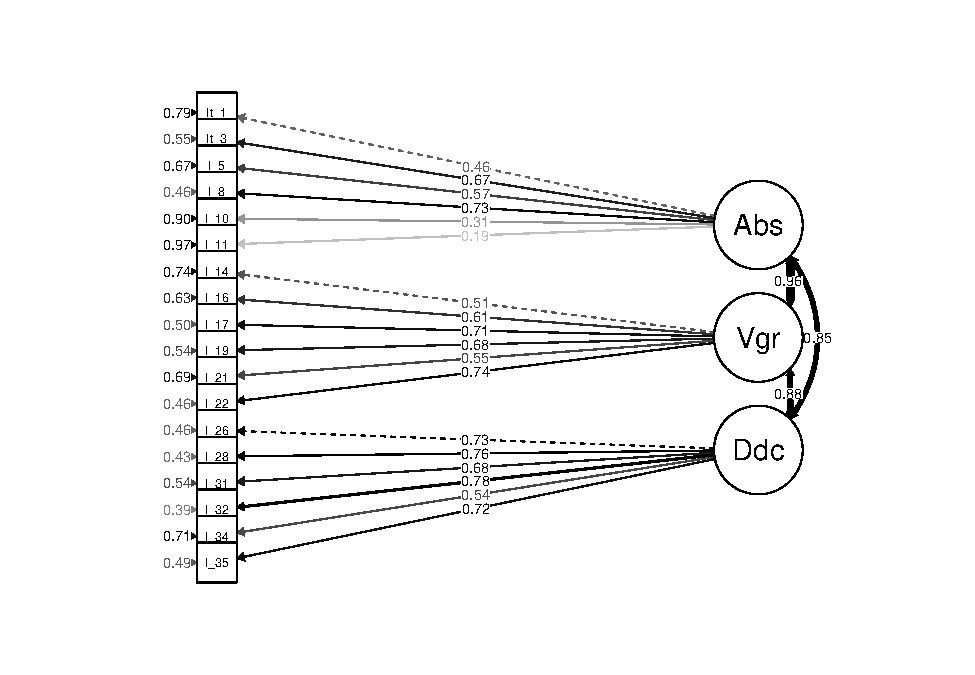
\includegraphics{SIOPpapaja_files/figure-latex/CFAatt1-1.pdf}
\caption{\label{fig:CFAatt1}Substantive factor measurement model}
\end{figure}

\begin{figure}
\centering
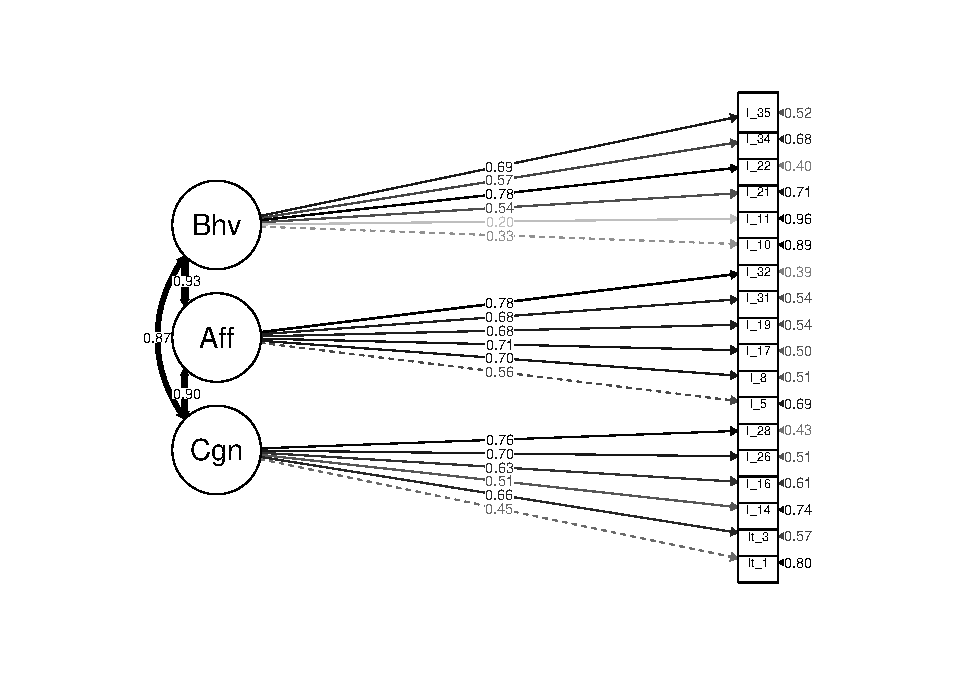
\includegraphics{SIOPpapaja_files/figure-latex/CFAatt2-1.pdf}
\caption{\label{fig:CFAatt2}Attitudinal factor measurement model}
\end{figure}

\begin{figure}
\centering
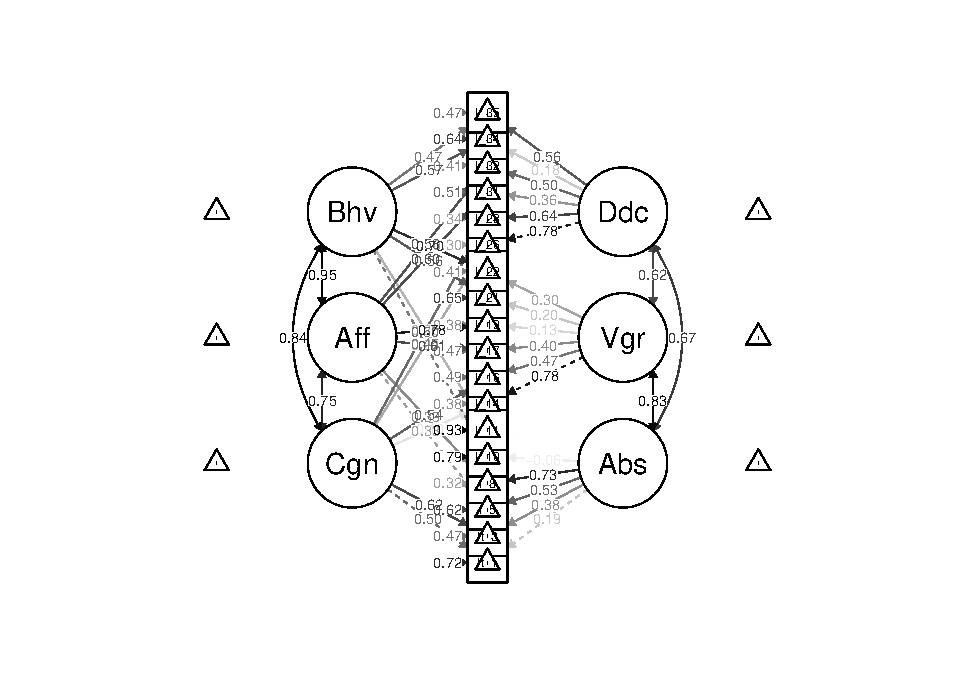
\includegraphics{SIOPpapaja_files/figure-latex/CFAatt3-1.pdf}
\caption{\label{fig:CFAatt3}Bifactor measurement model}
\end{figure}

\begin{table}[tbp]

\begin{center}
\begin{threeparttable}

\caption{\label{tab:fitmeasures}Summary fit statistics (18 item final proposed scale definitions)}

\begin{tabular}{llllllll}
\toprule
model & \multicolumn{1}{c}{Chi Square} & \multicolumn{1}{c}{df} & \multicolumn{1}{c}{RMSEA} & \multicolumn{1}{c}{SRMR} & \multicolumn{1}{c}{CFI} & \multicolumn{1}{c}{TLI} & \multicolumn{1}{c}{AIC}\\
\midrule
Attitudinal & 454.30 & 132.00 & 0.10 & 0.07 & 0.83 & 0.80 & 13,473.40\\
Substantive & 473.56 & 132.00 & 0.10 & 0.07 & 0.82 & 0.79 & 13,492.66\\
bifactor & 264.70 & 111.00 & 0.07 & 0.05 & 0.92 & 0.89 & 14,113.31\\
\bottomrule
\end{tabular}

\end{threeparttable}
\end{center}

\end{table}

\hypertarget{results}{%
\section{Results}\label{results}}

We used R {[}Version 4.1.0; R Core Team (2021){]} and the R-packages \emph{apaTables} {[}Version 2.0.8; Stanley (2021){]}, \emph{dplyr} {[}Version 1.0.6; Wickham et al. (2021){]}, \emph{DT} {[}Version 0.18; Xie et al. (2021){]}, \emph{forcats} {[}Version 0.5.1; Wickham (2021a){]}, \emph{ggplot2} {[}Version 3.3.3; Wickham (2016){]}, \emph{kableExtra} {[}Version 1.3.4; Zhu (2021){]}, \emph{labourR} {[}Version 1.0.0; Kouretsis et al. (2020){]}, \emph{lavaan} {[}Version 0.6.8; Rosseel (2012){]}, \emph{magrittr} {[}Version 2.0.1; Bache and Wickham (2020){]}, \emph{papaja} {[}Version 0.1.0.9997; Aust and Barth (2020){]}, \emph{purrr} {[}Version 0.3.4; Henry and Wickham (2020){]}, \emph{readr} {[}Version 1.4.0; Wickham and Hester (2020){]}, \emph{sem} {[}Version 3.1.11; Fox et al. (2020); Epskamp (2019){]}, \emph{semPlot} {[}Version 1.1.2; Epskamp (2019){]}, \emph{stringr} {[}Version 1.4.0; Wickham (2019){]}, \emph{tibble} {[}Version 3.1.2; Müller and Wickham (2021){]}, \emph{tidyr} {[}Version 1.1.3; Wickham (2021b){]}, and \emph{tidyverse} {[}Version 1.3.1; Wickham et al. (2019){]} for all analyses.

The eventual 18-item scale definitions identified via the two item reduction procedures are presented in Table XX. Subjecting these two structures to bifactor constraints was accomplished via full information maximum likelihood estimation, with the corrected item-total definition, somewhat surprisingly, resulting in a better fit (\(\chi^2\) = 227.89, RMSEA = 0.05, AIC = 14,050.98) than the CFA modification-index derived bifactor solution (\(\chi^2\) = 247.01, RMSEA = 0.06, AIC = 14,327.76).

\begin{table}[tbp]

\begin{center}
\begin{threeparttable}

\caption{\label{tab:scales}Final proposed scale definitions (derived via attendance to corrected item-total correlations or CFA modification indices)}

\begin{tabular}{llll}
\toprule
Substantive & \multicolumn{1}{c}{Attitudinal} & \multicolumn{1}{c}{Corrected.Item.Total.Definition} & \multicolumn{1}{c}{CFA.Modification.Index.Definition}\\
\midrule
Absorption & Cog &   Item\_1=`I’m able to concentrate on my work without distractions.`, &   Item\_2=`I have a hard time detaching mentally from my work.`,\\
Absorption & Cog &   Item\_3=`Time passes quickly while I’m working.`, &   Item\_3=`Time passes quickly while I’m working.`,\\
Absorption & Aff &   Item\_5=`I enjoy thinking about work even when I’m not at work.`, &   Item\_7=`I am happiest when I am immersed in a project.`,\\
Absorption & Aff &   Item\_8=`I love starting my workday.`, &   Item\_8=`I love starting my workday.`,\\
Absorption & Beh &   Item\_10=`I have to be reminded to take breaks while I’m at work.`, &   Item\_10=`I have to be reminded to take breaks while I’m at work.`,\\
Absorption & Beh &   Item\_9=`I devote more time than is expected of me.`, &   Item\_11=`I never miss a work deadline.`,\\
Vigor & Cog &   Item\_13=`I devote my full attention to my work tasks throughout the day.`, &   Item\_14=`Thinking about work saps my energy.`,\\
Vigor & Cog &   Item\_16=`I’m able to maintain good levels of energy throughout the workday.`, &   Item\_16=`I’m able to maintain good levels of energy throughout the workday.`,\\
Vigor & Aff &   Item\_17=`I enjoy spending time completing my job tasks.`, &   Item\_17=`I enjoy spending time completing my job tasks.`,\\
Vigor & Aff &   Item\_18=`Most days I feel enthusiastic about starting my work day.`, &   Item\_19=`I feel motivated to go beyond what is asked of me.`, [ADD "AT WORK"]\\
Vigor & Beh &   Item\_23=`I try my best to perform well at work.`, &   Item\_21=`When work is slow I find ways to be productive.`,\\
Vigor & Beh &   Item\_22=`I express enthusiasm for my job while at work.`, &   Item\_22=`I express enthusiasm for my job while at work.`,\\
Dedication & Cog &   Item\_26=`I believe this company cares about my career goals.`, &   Item\_26=`I believe this company cares about my career goals.`,\\
Dedication & Cog &   Item\_25=`I plan my future with this company.`, &   Item\_28=`This organization challenges me to work at my full potential.`,\\
Dedication & Aff &   Item\_31=`I feel proud of my accomplishments within this organization.`, &   Item\_31=`I feel proud of my accomplishments within this organization.`,\\
Dedication & Aff &   Item\_32=`My job makes me feel like I’m part of something meaningful.`, &   Item\_32=`My job makes me feel like I’m part of something meaningful.`,\\
Dedication & Beh &   Item\_33=`I make valued contributions to the organization.`, &   Item\_34=`I embrace challenging situations at work.`,\\
Dedication & Beh &   Item\_35=`I speak positively about this organization to others.`, &   Item\_35=`I speak positively about this organization to others.`,\\
\bottomrule
\end{tabular}

\end{threeparttable}
\end{center}

\end{table}

\hypertarget{final-scale-definitions-1}{%
\subsection{Final scale definitions}\label{final-scale-definitions-1}}

As alluded to above, rather than relying exclusively on empirical superiority, final scale definitions were also informed by considerations of content domain coverage, which slightly favored the CFA modification index-informed definition. Final scale \(\alpha\)'s were 0.66 (Absorption), 0.71 (Dedication), 0.65 (Vigor), 0.59 (Affect), 0.74 (Cognition), and 0.63 (Behavior). Correlations among unit-weighted scale aggregates are presented in Table XX.

\begin{lltable}

\begin{TableNotes}[para]
\normalsize{\textit{Note.} * p < 0.05; ** p < 0.01; *** p < 0.001}
\end{TableNotes}

\begin{longtable}{llllllll}\noalign{\getlongtablewidth\global\LTcapwidth=\longtablewidth}
\caption{\label{tab:unitweight}Unit-weighted scale intercorrelations (all conditions).}\\
\toprule
 & \multicolumn{1}{c}{1} & \multicolumn{1}{c}{2} & \multicolumn{1}{c}{3} & \multicolumn{1}{c}{4} & \multicolumn{1}{c}{5} & \multicolumn{1}{c}{$M$} & \multicolumn{1}{c}{$SD$}\\
\midrule
\endfirsthead
\caption*{\normalfont{Table \ref{tab:unitweight} continued}}\\
\toprule
 & \multicolumn{1}{c}{1} & \multicolumn{1}{c}{2} & \multicolumn{1}{c}{3} & \multicolumn{1}{c}{4} & \multicolumn{1}{c}{5} & \multicolumn{1}{c}{$M$} & \multicolumn{1}{c}{$SD$}\\
\midrule
\endhead
1. Absorption & - &  &  &  &  & 4.15 & 0.76\\
2. Vigor & .48*** & - &  &  &  & 4.49 & 0.72\\
3. Dedication & .66*** & .56*** & - &  &  & 3.97 & 0.87\\
4. Affect & .71*** & .75*** & .74*** & - &  & 3.72 & 0.81\\
5. Cognition & .75*** & .63*** & .86*** & .65*** & - & 4.25 & 0.82\\
6. Behavior & .72*** & .65*** & .71*** & .53*** & .61*** & 4.64 & 0.69\\
\bottomrule
\addlinespace
\insertTableNotes
\end{longtable}

\end{lltable}

\begin{quote}
For KULAS to do: two sections 1) 6x6 correlation matrix between scale scores 2) corrected item-total correlations
\end{quote}

\begin{table}[tbp]

\begin{center}
\begin{threeparttable}

\caption{\label{tab:final}}

\begin{tabular}{lllll}
\toprule
Number & \multicolumn{1}{c}{Item.text} & \multicolumn{1}{c}{Dimension.1} & \multicolumn{1}{c}{Dimension.2} & \multicolumn{1}{c}{Final}\\
\midrule
1 & I am able to concentrate on my work without distractions. & Absorption & Cognitive & Included\\
2 & I have a hard time detaching mentally from my work. & Absorption & Cognitive & \\
3 & Time passes quickly while I'm working. & Absorption & Cognitive & Included\\
4 & I find it difficult to mentally disconnect from work. & Absorption & Cognitive & \\
5 & I enjoy thinking about work even when I'm not at work. & Absorption & Affective & Included\\
6 & Most days, I feel happiest when the workday is soon to be complete. & Absorption & Affective & \\
7 & I am happiest when I am immersed in a project. & Absorption & Affective & \\
8 & I love starting my workday. & Absorption & Affective & Included\\
9 & I devote more time than is expected of me. & Absorption & Behavioral & Included\\
10 & I have to be reminded to take breaks while I'm at work. & Absorption & Behavioral & Included\\
11 & I never miss a work deadline. & Absorption & Behavioral & \\
12 & I never allow distractions to interfere with my work. & Absorption & Behavioral & \\
13 & I devote my full attention to my work tasks throughout the day. & Vigor & Cognitive & Included\\
14 & Thinking about work saps my energy. & Vigor & Cognitive & \\
15 & I would rather direct my focus toward a work task than a personal task. & Vigor & Cognitive & \\
16 & I'm able to maintain good levels of energy throughout the workday. & Vigor & Cognitive & Included\\
17 & I enjoy spending time completing my job tasks. & Vigor & Affective & Included\\
18 & Most days I feel enthusiastic about starting my work day. & Vigor & Affective & Included\\
19 & I feel motivated to go beyond what is asked of me. & Vigor & Affective & \\
20 & This job drains my energy. & Vigor & Affective & \\
21 & When work is slow I find ways to be productive. & Vigor & Behavioral & \\
22 & I express enthusiasm for my job while at work. & Vigor & Behavioral & Included\\
23 & I try my best to perform well at work. & Vigor & Behavioral & Included\\
24 & If I notice my energy level is low, I take corrective steps to re-energize. & Vigor & Behavioral & \\
25 & I plan my future with this company. & Dedication & Cognitive & Included\\
26 & I believe this company cares about my career goals. & Dedication & Cognitive & Included\\
27 & I often think about finding another job. & Dedication & Cognitive & \\
28 & This organization challenges me to work at my full potential. & Dedication & Cognitive & \\
29 & I am proud to be a member of this organization. & Dedication & Affective & \\
30 & I feel supported by my supervisor when I fail at a task. & Dedication & Affective & \\
31 & I feel proud of my accomplishments within this organization. & Dedication & Affective & Included\\
32 & My job makes me feel like I'm part of something meaningful. & Dedication & Affective & Included\\
33 & I make valued contributions to the organization. & Dedication & Behavioral & Included\\
34 & I embrace challenging situations at work. & Dedication & Behavioral & \\
35 & I speak positively about this organization to others. & Dedication & Behavioral & Included\\
36 & This organization provides the resources necessary for me to successfully perform my job. & Dedication & Behavioral & \\
\bottomrule
\end{tabular}

\end{threeparttable}
\end{center}

\end{table}

\hypertarget{discussion}{%
\section{Discussion}\label{discussion}}

\begin{quote}
\begin{enumerate}
\def\labelenumi{\arabic{enumi})}
\tightlist
\item
  methodological: bifactor structure
\item
  practical: public domain; scalable to 2 aggreggations
\item
  theoretical: possibly explains high inter-scale correlations reported on other measures
\end{enumerate}
\end{quote}

The purpose of this study was to document the development of an intentionally complex bifactor measure of engagement. To add an additional element of interest regarding the SIOP audience, we furthermore followed two divergent approaches that resulted in slightly different scale definitions. Surprisingly, the approach focusing on facet-level internal consistency maximization resulted in a better fitting CFA than did the approach focusing on CFA fit! Ultimately, differences were reconciled via qualitative consideration of content domain coverage, and the proposed 18-item final solution is a compromise between the two ``experimental'' models.

In addition to the information provided in this presentation, we have also documented evidence of convergent and discriminant validity of these scales, although the scope of that extends beyond a single SIOP presentation. We have a much larger technical report that documents the information in this paper as well as broader explorations of instrument criterion- and construct-validation and that technical report is currently published as an open-access document. Our items also intentionally carry no copyright and are freely available to any researcher or practitioner interested in the topic of engagment.

Our research contributes to theory in three key ways. Firstly, it introduces a novel measure of engagement, developed in English and available for free, that will allow future researchers to probe the tripartite attitudinal structure of the construct while at the same time measuring the more ``traditional'' structure. To our knowledge, ours is the only engagement scale that probes the specific attitudinal dimensions of engagement.

Secondly, we more generally advance the use of bifactor analysis as an alternative methodology for testing and comparing structural models of constructs that extends beyond investigations of common method variance. In the context of attitudinal constructs, it may be appropriate to examine the possibility of bifactor solutions that conform to attitudinal structure. We hope that this endeavor encourages other researchers to also extend the bifactor procedure to novel measurement pursuits.

Thirdly, we broaden our theoretical understanding of engagement. The unit-weighted inter-scale correlations exhibit only moderately high association (in the .6-ish range), which is promising and perhaps provides some support for retention of the 3-facet substantive model, which has been criticized for high observed inter-scale associations (e.g., see Kulikowski, 2017b). We show that a scale can be internally coherent while simultaneously measuring two different structural models. It is our hope that the success of this approach might evangelize bifactor analysis and the more general approach of consolidating and integrating models rather than parsing them.

\newpage

\hypertarget{references}{%
\section{References}\label{references}}

\begingroup
\setlength{\parindent}{-0.5in}
\setlength{\leftskip}{0.5in}

\hypertarget{refs}{}
\begin{CSLReferences}{1}{0}
\leavevmode\hypertarget{ref-alarcon2011relationship}{}%
Alarcon, G. M., \& Edwards, J. M. (2011). The relationship of engagement, job satisfaction and turnover intentions. \emph{Stress and Health}, \emph{27}(3), e294--e298.

\leavevmode\hypertarget{ref-R-papaja}{}%
Aust, F., \& Barth, M. (2020). \emph{{papaja}: {Create} {APA} manuscripts with {R Markdown}}. \url{https://github.com/crsh/papaja}

\leavevmode\hypertarget{ref-R-magrittr}{}%
Bache, S. M., \& Wickham, H. (2020). \emph{Magrittr: A forward-pipe operator for r}. \url{https://CRAN.R-project.org/package=magrittr}

\leavevmode\hypertarget{ref-baumruk2004missing}{}%
Baumruk, R. (2004). \emph{The missing link: The role of employee engagement in business success}. \emph{47}, 48--52.

\leavevmode\hypertarget{ref-caesens2014impact}{}%
Caesens, G., Stinglhamber, F., \& Luypaert, G. (2014). The impact of work engagement and workaholism on well-being: The role of work-related social support. \emph{Career Development International}.

\leavevmode\hypertarget{ref-R-semPlot}{}%
Epskamp, S. (2019). \emph{semPlot: Path diagrams and visual analysis of various SEM packages' output}. \url{https://CRAN.R-project.org/package=semPlot}

\leavevmode\hypertarget{ref-R-sem}{}%
Fox, J., Nie, Z., \& Byrnes, J. (2020). \emph{Sem: Structural equation models}. \url{https://CRAN.R-project.org/package=sem}

\leavevmode\hypertarget{ref-giordano_exploratory_2020}{}%
Giordano, C., Ones, D. S., Waller, N. G., \& Stanek, K. C. (2020). Exploratory bifactor measurement models in vocational behavior research. \emph{Journal of Vocational Behavior}, \emph{120}, 103430. \url{https://doi.org/10.1016/j.jvb.2020.103430}

\leavevmode\hypertarget{ref-girardi2019workaholism}{}%
Girardi, D., De Carlo, A., Dal Corso, L., Andreassen, C. S., \& Falco, A. (2019). Is workaholism associated with inflammatory response? The moderating role of work engagement. \emph{TPM-Testing, Psychometrics, Methodology in Applied Psychology}.

\leavevmode\hypertarget{ref-hanaysha2016testing}{}%
Hanaysha, J. (2016). Testing the effects of employee engagement, work environment, and organizational learning on organizational commitment. \emph{Procedia-Social and Behavioral Sciences}, \emph{229}, 289--297.

\leavevmode\hypertarget{ref-R-purrr}{}%
Henry, L., \& Wickham, H. (2020). \emph{Purrr: Functional programming tools}. \url{https://CRAN.R-project.org/package=purrr}

\leavevmode\hypertarget{ref-kahn1990psychological}{}%
Kahn, W. A. (1990). Psychological conditions of personal engagement and disengagement at work. \emph{Academy of Management Journal}, \emph{33}(4), 692--724.

\leavevmode\hypertarget{ref-kaiser_campbell_2019}{}%
Kaiser, F. G., \& Wilson, M. (2019). The campbell paradigm as a behavior-predictive reinterpretation of the classical tripartite model of attitudes. \emph{European Psychologist}, \emph{24}(4), 359--374. \url{https://doi.org/10.1027/1016-9040/a000364}

\leavevmode\hypertarget{ref-kaiser_campbell_2019}{}%
Kaiser, F. G., \& Wilson, M. (2019). The campbell paradigm as a behavior-predictive reinterpretation of the classical tripartite model of attitudes. \emph{European Psychologist}, \emph{24}(4), 359--374. \url{https://doi.org/10.1027/1016-9040/a000364}

\leavevmode\hypertarget{ref-R-labourR}{}%
Kouretsis, A., Bampouris, A., Morfiris, P., \& Papageorgiou, K. (2020). \emph{labourR: Classify multilingual labour market free-text to standardized hierarchical occupations}. \url{https://CRAN.R-project.org/package=labourR}

\leavevmode\hypertarget{ref-kulikowski_we_2017}{}%
Kulikowski, K. (2017a). Do we all agree on how to measure work engagement? Factorial validity of utrecht work engagement scale as a standard measurement tool - a literature review. \emph{International Journal of Occupational Medicine and Environmental Health}, \emph{30}(2), 161--175. \url{https://doi.org/10.13075/ijomeh.1896.00947}

\leavevmode\hypertarget{ref-kulikowski2017we}{}%
Kulikowski, K. (2017b). Do we all agree on how to measure work engagement? Factorial validity of utrecht work engagement scale as a standard measurement tool--a literature review. \emph{International Journal of Occupational Medicine and Environmental Health}, \emph{30}(2), 161--175.

\leavevmode\hypertarget{ref-R-tibble}{}%
Müller, K., \& Wickham, H. (2021). \emph{Tibble: Simple data frames}. \url{https://CRAN.R-project.org/package=tibble}

\leavevmode\hypertarget{ref-R-base}{}%
R Core Team. (2021). \emph{R: A language and environment for statistical computing}. R Foundation for Statistical Computing. \url{https://www.R-project.org/}

\leavevmode\hypertarget{ref-reise_rediscovery_2012}{}%
Reise, S. P. (2012). The rediscovery of bifactor measurement models. \emph{Multivariate Behavioral Research}, \emph{47}(5), 667--696. \url{https://doi.org/10.1080/00273171.2012.715555}

\leavevmode\hypertarget{ref-rich2010job}{}%
Rich, B. L., Lepine, J. A., \& Crawford, E. R. (2010). Job engagement: Antecedents and effects on job performance. \emph{Academy of Management Journal}, \emph{53}(3), 617--635.

\leavevmode\hypertarget{ref-rosenberg_cognitive_1960}{}%
Rosenberg, M. J. (1960). Cognitive, affective, and behavioral components of attitudes. In \emph{Attitude organization and change}.

\leavevmode\hypertarget{ref-R-lavaan}{}%
Rosseel, Y. (2012). {lavaan}: An {R} package for structural equation modeling. \emph{Journal of Statistical Software}, \emph{48}(2), 1--36. \url{https://www.jstatsoft.org/v48/i02/}

\leavevmode\hypertarget{ref-schaufeli2013engagement}{}%
Schaufeli, W. B. (2013). What is engagement? In \emph{Employee engagement in theory and practice} (pp. 29--49). Routledge.

\leavevmode\hypertarget{ref-schaufeli2003utrecht}{}%
Schaufeli, W. B., \& Bakker, A. B. (2003). Utrecht work engagement scale: Preliminary manual. \emph{Occupational Health Psychology Unit, Utrecht University, Utrecht}, \emph{26}(1), 64--100.

\leavevmode\hypertarget{ref-schaufeli_measurement_2002}{}%
Schaufeli, W. B., Salanova, M., González-Romá, V., \& Bakker, A. B. (2002). The measurement of engagement and burnout: A two sample confirmatory factor analytic approach. \emph{Journal of Happiness Studies}, \emph{3}(1), 71--92.

\leavevmode\hypertarget{ref-schaufeli_measurement_2002}{}%
Schaufeli, W. B., Salanova, M., González-Romá, V., \& Bakker, A. B. (2002). The measurement of engagement and burnout: A two sample confirmatory factor analytic approach. \emph{Journal of Happiness Studies}, \emph{3}(1), 71--92.

\leavevmode\hypertarget{ref-shaw2005engagement}{}%
Shaw, K. (2005). An engagement strategy process for communicators. \emph{Strategic Communication Management}, \emph{9}(3), 26.

\leavevmode\hypertarget{ref-R-apaTables}{}%
Stanley, D. (2021). \emph{apaTables: Create american psychological association (APA) style tables}. \url{https://CRAN.R-project.org/package=apaTables}

\leavevmode\hypertarget{ref-trogolo2020work}{}%
Trógolo, M. A., Morera, L. P., Castellano, E., Spontón, C., \& Medrano, L. A. (2020). Work engagement and burnout: Real, redundant, or both? A further examination using a bifactor modelling approach. \emph{European Journal of Work and Organizational Psychology}, \emph{29}(6), 922--937.

\leavevmode\hypertarget{ref-R-ggplot2}{}%
Wickham, H. (2016). \emph{ggplot2: Elegant graphics for data analysis}. Springer-Verlag New York. \url{https://ggplot2.tidyverse.org}

\leavevmode\hypertarget{ref-R-stringr}{}%
Wickham, H. (2019). \emph{Stringr: Simple, consistent wrappers for common string operations}. \url{https://CRAN.R-project.org/package=stringr}

\leavevmode\hypertarget{ref-R-forcats}{}%
Wickham, H. (2021a). \emph{Forcats: Tools for working with categorical variables (factors)}. \url{https://CRAN.R-project.org/package=forcats}

\leavevmode\hypertarget{ref-R-tidyr}{}%
Wickham, H. (2021b). \emph{Tidyr: Tidy messy data}. \url{https://CRAN.R-project.org/package=tidyr}

\leavevmode\hypertarget{ref-R-tidyverse}{}%
Wickham, H., Averick, M., Bryan, J., Chang, W., McGowan, L. D., François, R., Grolemund, G., Hayes, A., Henry, L., Hester, J., Kuhn, M., Pedersen, T. L., Miller, E., Bache, S. M., Müller, K., Ooms, J., Robinson, D., Seidel, D. P., Spinu, V., \ldots{} Yutani, H. (2019). Welcome to the {tidyverse}. \emph{Journal of Open Source Software}, \emph{4}(43), 1686. \url{https://doi.org/10.21105/joss.01686}

\leavevmode\hypertarget{ref-R-dplyr}{}%
Wickham, H., François, R., Henry, L., \& Müller, K. (2021). \emph{Dplyr: A grammar of data manipulation}. \url{https://CRAN.R-project.org/package=dplyr}

\leavevmode\hypertarget{ref-R-readr}{}%
Wickham, H., \& Hester, J. (2020). \emph{Readr: Read rectangular text data}. \url{https://CRAN.R-project.org/package=readr}

\leavevmode\hypertarget{ref-willmer_exploratory_2019}{}%
Willmer, M., Westerberg Jacobson, J., \& Lindberg, M. (2019). Exploratory and confirmatory factor analysis of the 9-item utrecht work engagement scale in a multi-occupational female sample: A cross-sectional study. \emph{Frontiers in Psychology}, \emph{10}. \url{https://doi.org/10.3389/fpsyg.2019.02771}

\leavevmode\hypertarget{ref-R-DT}{}%
Xie, Y., Cheng, J., \& Tan, X. (2021). \emph{DT: A wrapper of the JavaScript library 'DataTables'}. \url{https://CRAN.R-project.org/package=DT}

\leavevmode\hypertarget{ref-R-kableExtra}{}%
Zhu, H. (2021). \emph{kableExtra: Construct complex table with 'kable' and pipe syntax}. \url{https://CRAN.R-project.org/package=kableExtra}

\end{CSLReferences}

\endgroup


\end{document}
